\documentclass{article}
\usepackage{tikz}
\usetikzlibrary{automata,positioning}

\begin{document}

\begin{figure}[h]
    \centering
    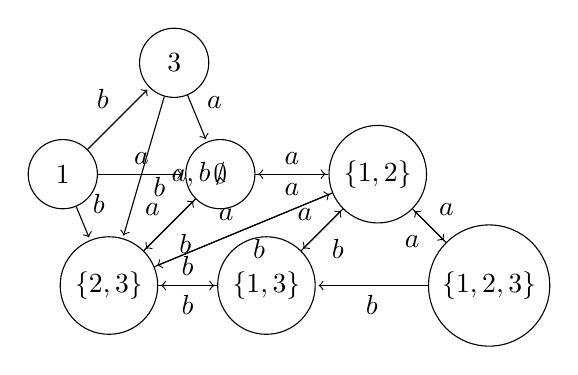
\begin{tikzpicture}[shorten >=1pt,node distance=2cm,on grid,auto]
        % States
        \node[state] (q_0) {$\emptyset$};
        \node[state] (q_1) [left of=q_0] {1};
        \node[state] (q_2) [above right of=q_1] {3};
        \node[state] (q_3) [right of=q_0] {$\{1, 2\}$};
        \node[state] (q_4) [below right of=q_3] {$\{1, 2, 3\}$};
        \node[state] (q_5) [below left of=q_3] {$\{1, 3\}$};
        \node[state] (q_6) [left of=q_5] {$\{2, 3\}$};

        % Edges
        \path[->]
            (q_0) edge node {$a, b$} (q_0)
            (q_0) edge node {$b$} (q_6)
            (q_0) edge node {$a$} (q_3)
            (q_1) edge node {$a$} (q_0)
            (q_1) edge node {$b$} (q_6)
            (q_1) edge node {$b$} (q_2)
            (q_2) edge node {$a$} (q_0)
            (q_2) edge node {$b$} (q_6)
            (q_3) edge node {$a$} (q_0)
            (q_3) edge node {$b$} (q_6)
            (q_3) edge node {$a$} (q_4)
            (q_3) edge node {$b$} (q_5)
            (q_4) edge node {$a$} (q_3)
            (q_4) edge node {$b$} (q_5)
            (q_5) edge node {$a$} (q_3)
            (q_5) edge node {$b$} (q_6)
            (q_6) edge node {$a$} (q_3)
            (q_6) edge node {$b$} (q_5)
            (q_6) edge node {$a$} (q_0);
    \end{tikzpicture}
    \caption{Si on supprime les états qui ne peuvent être atteints, on obtient l'AFD suivant :}
\end{figure}

\begin{figure}[h]
    \centering
    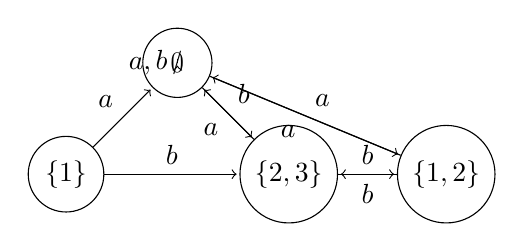
\begin{tikzpicture}[shorten >=1pt,node distance=2cm,on grid,auto]
        % States
        \node[state] (q_0) {$\emptyset$};
        \node[state] (q_1) [below left of=q_0] {$\{1\}$};
        \node[state] (q_2) [below right of=q_0] {$\{2, 3\}$};
        \node[state] (q_3) [right of=q_2] {$\{1, 2\}$};

        % Edges
        \path[->]
            (q_0) edge node {$a, b$} (q_0)
            (q_0) edge node {$b$} (q_2)
            (q_0) edge node {$a$} (q_3)
            (q_1) edge node {$a$} (q_0)
            (q_1) edge node {$b$} (q_2)
            (q_2) edge node {$a$} (q_0)
            (q_2) edge node {$b$} (q_3)
            (q_3) edge node {$a$} (q_0)
            (q_3) edge node {$b$} (q_2);
    \end{tikzpicture}
    \caption{Le langage que cet automate accepte est le suivant : $\{b(ab)^n : n \in \mathbb{N}\}$}
\end{figure}

\end{document}